
\documentclass{article}
\usepackage[utf8]{inputenc}


\title{TACOS}
\author{Julien ALAIMO, Hugo FEYDEL, Olivier HUREAU }
\date{2019-2020}
\usepackage{graphicx}
\usepackage{listings}
\lstset{language=C}
\setlength{\marginparwidth}{20pt}
\begin{document}

\maketitle

\section{Fonctionnalités intéressante/importante}

TACOS (The Amazing Control Operating System) est un système d'exploitation incomplet mais robuste : il dispose d'un système de multithreading complet et d'un système de fichier opérationnel. Il est également livré avec les fonctionnalités basiques d'entrées/sorties (cf. 2.1).

\subsection{Le Multithreading}

Le multiThreading permet à un utilisateur de faire tourner plusieurs instructions en parallèle. Similaire au processus dans un environement linux, les threads partagent le même espace mémoire.

Notre réalisation permet une utilisation simpliste et permissive du multithreading : si certaines mécaniques de fermeture sont oublié, le système le fera par lui même. 

\subsection{Le Système de fichier}

Le système de fichier fourni permet à l'utilisateur de se déplacer à sa guise dans l'arborescence, de créer/supprimer des répertoires et des fichiers, d'ouvrir des fichiers, de lire leur contenu ou le modifier.

Il est possible d'utiliser des noms de chemins (absolus comme relatifs) et les répertoires spéciaux "." (répertoire courant), ".." (répertoire parent) et "/" (répertoire racine).

Attention, ce système de fichier opère sur des fichiers de tailles fixes uniquement.

\newpage

\section{Spécifications}

\subsection{Entrées/Sorties}
\begin{itemize}
    \item 
    \textbf{void PutChar(char c);}
    
    Ecrit le caractère \textbf{c}  sur la sortie standard
    
    \item 
    \textbf{void PutString(char * string);}
    
    Ecrit la chaîne de caractères \textbf{string} sur la sortie standard.
    La chaîne de caractères doit finir par '\textbackslash0'.
    La taille maximale de la chaîne de caractères est définie par la constante \textbf{MAX\_STRING\_SIZE} (cf. "system.h").

    L'appel système \textbf{PutString} est moins coûteux que plusieurs appels système \textbf{PutChar}.
    
     \item 
    \textbf{int GetChar();}
    
    Retourne la valeur ascii d'un caractère rentré dans l'entrée standard.
    La fonction attend qu'un caractère soit disponible, elle est bloquante.
    
    
     \item 
    \textbf{void GetString(char * string, int taille);}
    
    Ecrit la chaîne de caractères rentrée dans l'entrée standard à l'adresse de la chaîne de caractères passée en paramètre \textbf{string}. La taille de cette chaîne de caractère sera inférieure ou égale au paramètre \textbf{taille}. Si celle de la chaîne rentrée lui est supérieure, la chaîne obtenue en sera une troncature.
    
      \item 
    \textbf{void GetInt(int * n);}
    
    Ecrit l'entier rentré dans l'entrée standard à l'adresse pointée par le paramètre \textbf{n}.
    L'entier peut être positif comme négatif.
    La valeur absolue de l'entier ne doit pas être supérieure à \[10^{10}-1\] (valeur absolue). Sinon une erreur est levée.
    
    
    
      \item 
    \textbf{void PutInt(int n);}
    
     Ecrit l'entier en paramètre \textbf{int n} sur la sortie standard
    L'entier peut être positif comme négatif.
    La valeur absolue de l'entier ne doit pas être supérieure à \[10^{10}-1\] (valeur absolue). Sinon une erreur est levée.
    
    
\end{itemize}

\newpage

\subsection{Threads}
Le programmation multithreadé permet à l'utilisateur d'éxecuter plusieurs threads simultanément. Les threads partagent la mémoire virtuelle et l'utilisation du coeur. Chaque thread possède néanmoins son propre fil d'exécution, ses propres registres (dont le pointeur d'instrcution PC) et sa pile.


Tout les threads sont identifié par des identifiants unique stocké sur des unsigned int. A la mort de chaque thread, lors de la mort de son parent, l'identifiant du thread enfant est retransmis au système de gestion des identifiants afin qu'il soit recyclé. Le thread principal ayant pour identifiant '1', si la mémoire le permet, il est possible d'utiliser jusqu'à \(2^{32}-1\) thread simultanément mais aussi possible d'avoir une infinité de thread ayant était éxecuté sur la machine d'un point de vue temporel.

Dans le système tacOS il existe un lien de parenté entre tout les threads. Chaque thread créé est enfant du thread créateur. A la fin de l'exécution d'un thread dis \textit{\textbf{parent}} , celui-ci va attendre la fin de l'exécution de tout ses fils. 

Cependant, un mode \textit{\textbf{survivant}} est mis en place tel que lorsqu'un un thread est dis \textit{\textbf{survivant}}, il ne seras pas attendu pas son thread père met par son grand père. 

Voici les différentes procédures liéé aux threads :
\begin{itemize}
 
    \item 
    \textbf{unsigned int CreateThread(void * f (void * arg), void * arg;}
    
    Crée un thread utilisateur et lance la routine \textbf{f}. Le deuxième argument 
    \textbf{void * arg} est passé en argument a la fonction f.
    Retourne l'identifiant du thread.
   
   \item 
   \textbf{void ExitThread(void * obj)} 
   
   Termine le thread courant et injecte l'adresse de l'objet dans les structures l'adresse \textbf{void * obj} afin qu'un thread parent puisse l'utiliser. Doit être appelé lorsque l'on désire terminer un thread "fils". \textit{Le système possède néanmoins un mécanisme permettant de rattraper cet oubli }
   
   \item 
   \textbf{unsigned int ThreadId();}
   
  Retourne l'identifiant du thread courant.   
   
   \item
   \textbf{void * WaitForChildExited(int CID);} 
   
   Attente passif que le thread d'identifiant \textbf{CID} termine. Retourne une adresse correspondant à l'objet donné par le thread enfant lors de son exit. Si cette adresse est équivalente à \textbf{(void *) -1}, alors l'identifiant \textbf{CID} n'as pas était reconnu où le thread n'est pas enfant.
   
    
\end{itemize}


\begin{itemize}
  \item 
  \textbf{void WaitForAllChildExited();}
  
  Met le thread en attente actif. Le thread sort de l'attente quand plus aucun de ses threads enfants sont en cours d'execution (y compris les thread en mode survivant)
  
  \item 
  \textbf{int StopChild(int CID)}
  
  Met en pause le thread enfant d'identifiant \textbf{CID}. 
  La fonction retourne :    
    \begin{itemize}
      \item \textbf{0} Si succès
      \item \textbf{1} Si l'arrêt à échoué
      \item \textbf{2} Si l'identifiant n'est pas celui d'un de ses enfants
    \end{itemize} 
    Si le thread est en zone critique (Ecriture /lecture) dans la conssole, le thread s'arretera après cette lecture/ecriture.      
    
  
  \item 
  \textbf{int WakeUpChild(int CID);}
  
    
  Reveil le thread enfant d'identifiant \textbf{CID}. 
  La fonction retourne :    
    \begin{itemize}
      \item \textbf{0} Si succès
      \item \textbf{1} Si l'identifiant n'est pas celui d'un de ses enfants
      \item \textbf{2} Si le thread n'est pas en pause
    \end{itemize} 
    
  
  \item 
  \textbf{int makeChildSurvive(int CID);}
  
  Met le thread enfant d'identifiant \textbf{CID} en \textbf{mode survivor} jusqu'à la mort du père .
  
  \item 
  \textbf{void makeAllChildSurvive();}
  
  Met tout les threads enfant en \textbf{mode survivor} jusqu'à la mort du père courant.
\end{itemize}

\subsection{Système de fichiers}

\begin{itemize}

\item
Fonctions de navigation/création/suppression sur l'arborescence :

Les fonctions \textbf{Create()} et \textbf{Remove()} opèrent depuis le répertoire courant.

\begin{itemize}

  \item
  \textbf{bool Create(const char *name, int initialSize, File\_type type = f);}

  Crée un fichier ou un répertoire selon le type \textbf{type} (f pour fichier, d pour répertoire, fixé à f par défaut), de nom \textbf{name} et de taille \textbf{initialSize}.
  Retourne vrai si succès, faux si le fichier/répertoire existe déjà ou si l'espace disponible est insuffisant.

    \item
    \textbf{ bool Remove(const char *name, unsigned int tid = 0);}

    Supprime un fichier de nom \textbf{name} du thread d'identifiant \textbf{tid}.

    Retourne vrai si succès, faux si le fichier n'existe pas.

\end{itemize}

Les fonctions \textbf{OpenFromPathName()},  \textbf{MkdirFromPathName()} et  \textbf{RmdirFromPathName()} utilisent la fonction  \textbf{CdFromPathName()} afin de se placer dans le bon répertoire, effectuer leurs opérations, et enfin de se replacer dans le répertoire avant les changements.

     \begin{itemize}

     \item
      \textbf{path\_parse\_t * CdFromPathName(const char *path\_name, unsigned int tid = 0, int truncate = 0);}

     Change le répertoire courant avec celui de nom du dernier élément de \textbf{path\_name} du thread d'identifiant \textbf{tid} et retourne un pointeur vers une structure  \textbf{path\_parse\_t}.

     Exemple :

     CdFromPathName("/folder1/folder2") vous placera dans "folder2" si la racine contient "folder1", NULL sinon.

     \item
     \textbf{bool MkdirFromPathName(const char* path\_name, unsigned int tid = 0);}

  Crée un répertoire de nom du dernier élément de \textbf{path\_name} du thread d'identifiant \textbf{tid} dans le répertoire de nom de l'avant dernier élément de  \textbf{path\_name}.

  Retourne vrai si succès, faux si chemin incorrect ou si le répertoire existe déjà ou si l'espace disponible est insuffisant.

  Exemples :

  MkdirFromPathName("folder1/folder2/file1") renverra false.

  MkdirFromPathName("folder2/folder3") créera "folder3" dans "folder2" en admettant que le répertoire courant le contienne.

  MkdirFromPathName("/folder3") créera "folder3" à la racine.

 	\item
 	\textbf{bool RmdirFromPathName(const char* path\_name, unsigned int tid = 0);}

  Supprime un répertoire de nom du dernier élément de \textbf{path\_name} du thread d'identifiant \textbf{tid} dans le répertoire de nom de l'avant dernier élément de  \textbf{path\_name}.

  Retourne vrai si succès, faux si le répertoire n'existe pas ou si le répertoire n'est pas vide.


\end{itemize}

\item

Fonctions utilisateurs :

\begin{itemize}

	\item
    \textbf{int UserOpen(const char *name, unsigned int tid);}

	Ouvre un fichier de nom du dernier élément de \textbf{name} du thread d'identifiant \textbf{tid} et retourne l'entier du descripteur de fichier associé (-1 si échec).

	\item
    \textbf{int UserRead(int fileDescriptor, char *into, int numBytes, unsigned int tid);}

	Lit \textbf{numBytes} octets depuis le fichier décrit par \textbf{fileDescriptor} et les écrit dans \textbf{into}.

    \item
    \textbf{int UserWrite(int fileDescriptor, char *from, int numBytes, unsigned int tid);}

	Ecrit \textbf{numBytes} octets depuis \textbf{from} dans le fichier décrit par \textbf{fileDescriptor}.

    \item
    \textbf{void UserSetSeek(int fileDescriptor, int position, unsigned int tid);}

	Change la position du curseur dans l'entête du fichier décrit par \textbf{fileDescriptor} par \textbf{position}.

    \item
    \textbf{int UserCloseFile(int fileDescriptor, unsigned int tid);}

	Ferme le fichier décrit par \textbf{fileDescriptor}.

\end{itemize}

\end{itemize}

\newpage

\newpage
\section{Tests Utilisateurs}
\textit{une partie "tests utilisateurs" décrivant les programmes de test que vous avez réalisés, ce qu'ils montrent, ...}
\vspace{5mm}

\subsection{Threads}

\begin{itemize}
	\item Le test de la class \textit{\textbf{ List} (que nous avons modifié)} se lance avec l'argument -tl. Ce test va vérifier si : Un liste retourne le bon boolean lors de l'appel de IsEmpty(), les éléments ont bien était ajouté dans le bon ordre, les éléments ont bien était supprimé dans le bon ordre, la fonction ajouté get(index) fonctionne correctement. \textit{voir testImplem.cc}


\item Le test de la class \textbf{UserThreadManagerId} se lance avec l'argument -utmmono. Ce test va vérifier si : Le manager commence au bon endroit, les identifiants sont recyclés, un identifiant recyclé est donné en priorité par rapport à un nouvel indentifiant. \textit{voir testImplem.cc}

\item \textbf{CreateAndReturn.c} : Ce test vérifie qu'un Thread se crée correctement et que sa valeur de retour est juste.

\item \textbf{ExitWithoutStatement.c} : Ce test vérifie que même lorsqu'un thread n'utilise pas d'appel de retour (return ou ExitThread), celui-ci se termine correctement.

\item \textbf{MultiGetChar.c} : Ce test vérifie la spécification de la console and mode multithreadé : Plusieurs getString sont lancé en même temps, on vérifie que l'execution de celle-ci est bien de manière séquentiel.


\item \textbf{Survive.c} : Ce test vérifie que l'implémentation du mode survivor fonctionne correctement. Le fils doit écrire sur le terminal avec que le petit fils ait finis d'écrire.

\item \textbf{WaitForThread.c} : Ce test vérifie que les parents attendent bien que leurs fils se terminent (un seul père, 2 fils)

\item \textbf{WaitForThreadMulti.c} : Ce test vérifie que les parents attendent bien que leurs fils se terminent (un seul père, 1 fils, 1 petit fils)

		\item \textbf{Sleep.c} : Ce test vérifie qu'un thread père peux bien mettre en attente un fils : Le fils est programmé pour ecrire en continu sur la console, le StopThread() arrète donc bien l'enfant de parler.

\item \textbf{Wake.c} :	Ce test vérifie père peux bien réveiller son fils.




\end{itemize}

\newpage

\section{Implémentation}

\vspace{5mm}

\subsection{Threads}




Pour implémenter les threads, nous avons choisis d'utiliser les 3 classes suivantes : UserThread, ManagerUserThreadID,UserThreadData

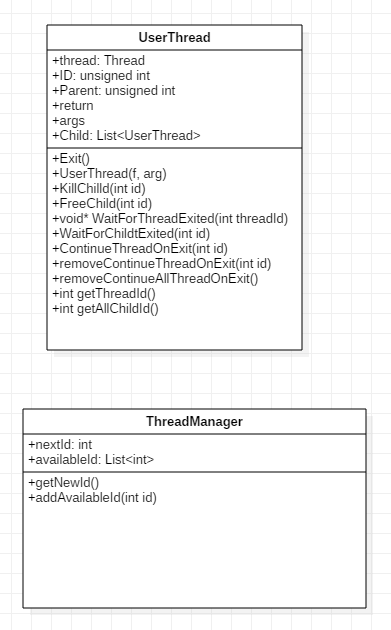
\includegraphics[scale=0.7]{code/userprog/UserThread.PNG}

L'adresse d'un UserThread est stocké dans la class Thread, Ainsi, le UserThread du currentThread est acessible via currentThread-$>$getAdressOfUserThread(). En ayant accès au UserThread, on a donc les informations nécessaire sur le thread tel que : Les UserThreadData de tout ses fils, le UserThread du père, l'identifiant est toutes autres informations nécessaire.
	
\vspace{5mm} 

Nous avons choisis de créer une nouvelle classe afin de gagner en lisibilité au niveau du code. De plus, cet implémentation est certes gourmandes en mémoire mais permet d'effectuer des tâches plus rapidement. Il aurais était possible d'utiliser un arbre de UserThread mais la recherche du UserThread correspondant à chaque thread aurais était beaucoup trop longue.



La création du Thread utilisateur se fait alors par le biai du constructeur de la classe UserThread. Lors de la construction un "new Thread()" est appelé. 



Le terminaison des threads sans fonction de retour ou ExitThread() se fait par l'appel du syscall ExitThread stocké dans le registre RA (31) de chaque thread dès son initialisation.

La destruction des classes Thread se fait lors de l'appel d'un WaitChildExited(unsigned int CID). Lors de cette appel, le père essaye de prendre un sémaphore du UserThread fils (token rajouté lors du ExitThread() , récupèrer l'adresse de retour du fils et détruire les différentes classes.

L'assignation des identifiants d'UserThread se fait via le UserThreadManager.

\subsection{Système de fichiers}
\begin{itemize}
\item
Le Système de fichiers est organisé de la manière suivante :
\begin{itemize}
	\item
	Une table globale des fichiers ouverts sous forme de liste chaînée (cf.  \textbf{global\_file\_table\_t}).
	\item
	Une table des fichiers ouverts par thread sous forme de liste chaînée (cf \textbf{file\_table\_t}). Les 2 premiers élément de l'OpenFileTable de chaque thread sont dédiés aux répertoires racine (indice 0) et courant (indice 1).

\end{itemize}

 \begin{lstlisting}[frame=single]
typedef struct global_file_table {
    OpenFile *openFile;
    struct global_file_table *next;
} global_file_table_t;
  \end{lstlisting}

  \begin{lstlisting}[frame=single]
typedef struct file_table {
    unsigned int tid;
    char *path;
    OpenFile** OpenFileTable;
    struct file_table *next;
} file_table_t;
  \end{lstlisting}

 \item
La fonction "CdFromPathName"  découpe le nom de chemin par le séparateur "/" en tableau de chaînes de caractères (stockée dans \textbf{pathSplit}) afin de le parcourir répertoire par répertoire (en changeant le répertoire courant) jusqu'à (\textbf{size} - \textbf{truncate}) et retourne un pointeur vers une  structure \textbf{path\_parse\_t} (cf. ci-après).


  \begin{lstlisting}[frame=single]
  typedef struct path_parse {
    char** pathSplit;
    int size;
} path_parse_t;
  \end{lstlisting}

  Exemple :
  En admettant que "folder1" existe dans le répertoire courant, CdFromPathName("folder1/folder2/file1", 1) vous placera dans "folder2" et renverra un pointeur vers une structure suivante avec les champs suivants :
  pathSplit = [ [folder1] [folder2] ] ; size = 2.

 \end{itemize}

\section{Scolaire}
\textit{une partie plus "scolaire" où vous décrivez l'organisation de votre travail (planning, ...), commentaires constructifs sur le déroulement du projet, ...}
\vspace{5mm}

\end{document}
